\documentclass[conference]{IEEEtran}
\IEEEoverridecommandlockouts
\usepackage{amsmath,amssymb,amsfonts}
\usepackage{graphicx}
\usepackage{textcomp}
\usepackage{xcolor}
\usepackage{float}
\usepackage{cite}
\usepackage[bookmarks=false]{hyperref}
\usepackage{algorithm}
\usepackage{algorithmic}
\usepackage[portuguese]{babel}



\def\BibTeX{{\rm B\kern-.05em{\sc i\kern-.025em b}\kern-.08em
    T\kern-.1667em\lower.7ex\hbox{E}\kern-.125emX}}
\begin{document}

\makeatletter
\def\IEEEkeywordsname{Palavras-chave} % muda "Index Terms" para "Palavras-chave"
\renewcommand{\abstractname}{Resumo} % muda "Abstract" para "Resumo"
\renewcommand{\refname}{Referências}
\renewcommand{\tablename}{TABELA}
\renewcommand{\algorithmicrequire}{\textbf{Entrada:}}
\renewcommand{\algorithmicensure}{\textbf{Saída:}}
\renewcommand{\algorithmicreturn}{\textbf{retorna:}}
\renewcommand{\algorithmiccomment}[1]{\hfill \textit{#1}}
\renewcommand{\listalgorithmname}{Lista de Algoritmos} % opcional, para lista
\renewcommand{\algorithmname}{Algoritmo}
\makeatother


\title{Objetos Celestes: Uma análise exploratória\\

}

\author{\IEEEauthorblockN{1\textsuperscript{º} Carlos Vinicius S. Mesquita}
\IEEEauthorblockA{\textit{dept. de Engenharia de Teleinformática} \\
\textit{Universidade Federal do Ceará}\\
Fortaleza, Brasil \\
carlos.mesquita12@alu.ufc.br}
\and
\IEEEauthorblockN{2\textsuperscript{º} Francisco Vinicius Castro Silveira}
\IEEEauthorblockA{\textit{dept. de Engenharia de Teleinformática} \\
\textit{Universidade Federal do Ceará}\\
Fortaleza, Brasil \\
viniciuscastro2615@alu.ufc.br}
\and
\IEEEauthorblockN{3\textsuperscript{º} Thiago Siqueira de Sousa}
\IEEEauthorblockA{\textit{dept. de Engenharia de Teleinformática} \\
\textit{Universidade Federal do Ceará}\\
Fortaleza, Brasil \\
thiago.siqueira@alu.ufc.br}
}


\maketitle

\begin{abstract}
[A FAZER] Lorem ipsum dolor sit amet, consectetur adipiscing elit, sed do eiusmod tempor incididunt ut labore et dolore magna aliqua. Ut enim ad minim veniam, quis nostrud exercitation ullamco laboris nisi ut aliquip ex ea commodo consequat. Duis aute irure dolor in reprehenderit in voluptate velit esse cillum dolore eu fugiat nulla pariatur. Excepteur sint occaecat cupidatat non proident, sunt in culpa qui officia deserunt mollit anim id est laborum. Sed ut perspiciatis unde omnis iste natus error sit voluptatem accusantium doloremque laudantium, totam rem aperiam, eaque ipsa quae ab illo inventore veritatis et quasi architecto beatae vitae dicta sunt explicabo. Nemo enim ipsam voluptatem quia voluptas sit aspernatur aut odit aut fugit, sed quia consequuntur magni dolores eos qui ratione voluptatem sequi nesciunt. Neque porro quisquam est, qui dolorem ipsum quia dolor sit amet, consectetur, adipisci velit, sed quia non numquam eius modi tempora incidunt ut labore et dolore magnam aliquam quaerat voluptatem.
\end{abstract}
\vspace{5pt}
\begin{IEEEkeywords}
 SDSS DR17, galáxias, estrelas, quasares, EDA
\end{IEEEkeywords}

\section{Introdução}

Galáxias, estrelas e quasares são objetos celestes centrais na astronomia, pois representam diferentes estágios e fenômenos fundamentais no universo. As galáxias constituem vastos sistemas gravitacionalmente ligados, formados por bilhões de estrelas, gás e poeira, que evoluem ao longo de bilhões de anos. Os quasares (quasi-stellar objects, QSO) correspondem a núcleos galácticos extremamente luminosos, cuja emissão de energia é alimentada pela acreção de matéria em torno de buracos negros supermassivos \cite{b1}. Já as estrelas são corpos luminosos compostos principalmente por hidrogênio e hélio, onde ocorrem reações de fusão nuclear responsáveis pela geração de energia e pela síntese dos elementos químicos que enriquecem o Universo \cite{b2}.

O estudo desses corpos celestes requer coleta massiva de dados, obtidos por meio de instrumentos de alta precisão, como fibras ópticas, filtros fotométricos, câmeras e telescópios \cite{b3}. Esses dispositivos possibilitam a geração de conjuntos de dados detalhados que descrevem características físicas dos objetos observados, em formatos que variam entre imagens, tabelas, séries temporais e arquivos específicos da área, como os arquivos FITS (Flexible Image Transport System) \cite{b4}. Nesse contexto, o Sloan Digital Sky Survey (SDSS) destaca-se como uma das iniciativas mais importantes da astronomia moderna, sendo responsável por alguns dos mais completos catálogos estelares do mundo. O dataset utilizado neste estudo pertence ao Data Release 17 (DR17) do SDSS e contém informações fotométricas e de posicionamento sobre galáxias, estrelas e quasares. As observações foram realizadas com o telescópio de 2,5 metros localizado no Apache Point Observatory, EUA, equipado com uma câmera composta por 30 sensores CCD dispostos em seis colunas e operando em modo de varredura contínua, o que possibilitou registrar imagens precisas nos cinco filtros fotométricos u, g, r, i e z \cite{b3}.
\subsection{Trabalhos Relacionados}
Estudos posteriores com dados do SDSS têm se concentrado principalmente no desenvolvimento de modelos de classificação de galáxias, estrelas e quasares utilizando machine learning e deep learning. Veloso, Júnior e Rego \cite{b5} propõem uma rede multicamadas de perceptrons utilizando 17 variáveis do dataset para classificação de corpos celestes. Os trabalhos \cite{b6, b7, b8} focam em variáveis fotométricas como preditores em seus modelos de classificação. Esses estudos, assim como outros na literatura, concentram-se principalmente no desempenho preditivo dos modelos em detrimento da análise exploratória, que, quando realizada, limita-se a técnicas básicas. 


Este trabalho busca preencher essa lacuna ao realizar uma análise exploratória aprofundada dos dados do SDSS DR17. Aplicando técnicas univariadas, bivariadas e multivariadas, investigamos a distribuição de características individuais, relações entre variáveis e análise envolvendo múltiplos atributos. Essa abordagem visa compreender melhor a estrutura e qualidade dos dados, identificando tendências, outliers e correlações relevantes que possam fundamentar futuros preprocessamentos para modelos de regressão e classificação.

\section{Métodos}

Os métodos de análise exploratória empregados organizam-se em três fases. A primeira consiste na análise univariada, que examina individualmente cada variável por meio de estatísticas descritivas e visualizações em histogramas e boxplots, conduzida em abordagens incondicional e condicional às classes. A segunda fase é a análise bivariada, que investiga relações entre pares de variáveis através de scatterplots e matriz de correlação. Por fim, aplica-se a Análise de Componentes Principais (PCA), uma técnica para analisar os dados de modo multivariado.

O trabalho foi desenvolvido em linguagem Python devido ao seu ecossistema voltado à EDA. Bibliotecas utilizadas foram Pandas para manipulação dos dados, NumPy para operações matriciais, Matplotlib e Seaborn para visualização.


\subsection{Desrição do Dataset}

O conjunto de dados bruto é tabular e estruturado em 18 colunas e 100000 amostras não duplicadas de corpos celestes. A tabela \ref{tab:descrição_colunas} informa com mais detalhes o que cada coluna do dataset representa. Podemos ver que os dados se dividem em: variáveis de identificação ({\tt obj\_ID},  {\tt spec\_obj\_ID}), de posição ({\tt alpha}, {\tt delta}), variáveis fotométricas observadas ({\tt u}, {\tt g}, {\tt r}, {\tt i}, {\tt z} e {\tt redshift}) e variáveis referentes ao telescópio ({\tt plate}, {\tt cam\_col}, etc.).

\begin{table}[H]
\centering
\caption{Descrição das colunas do conjunto de dados SDSS DR17.}
\label{tab:descrição_colunas}
\resizebox{\columnwidth}{!}{%
\begin{tabular}{l|l}
\hline
\textbf{Coluna} & \textbf{Descrição} \\ 
\hline
\texttt{obj\_ID} & Identificador único do objeto no catálogo de imagens. \\ 
\texttt{alpha} & Ascensão Reta (Right Ascension) em coordenadas equatoriais. \\ 
\texttt{delta} & Declinação (Declination) em coordenadas equatoriais. \\ 
\texttt{u} & Magnitude no filtro ultravioleta (u). \\ 
\texttt{g} & Magnitude no filtro verde (g). \\ 
\texttt{r} & Magnitude no filtro vermelho (r). \\ 
\texttt{i} & Magnitude no filtro infravermelho próximo (i). \\ 
\texttt{z} & Magnitude no filtro infravermelho (z). \\ 
\texttt{run\_ID} & Número da varredura do telescópio. \\ 
\texttt{rerun\_ID} & Identifica o processamento da imagem. \\ 
\texttt{cam\_col} & Coluna da câmera (CCD). \\ 
\texttt{field\_ID} & Campo observado. \\ 
\texttt{spec\_obj\_ID} & Identificador único do objeto no catálogo espectroscópico. \\ 
\texttt{class} & Classe: galáxia, estrela ou quasar. \\ 
\texttt{redshift} & Desvio para o vermelho medido. \\ 
\texttt{plate} & Identificador da placa espectroscópica. \\ 
\texttt{MJD} & Data Juliana Modificada da captura. \\ 
\texttt{fiber\_ID} & Fibra óptica usada na captura. \\ 
\hline
\end{tabular}%
}
\end{table}

Para este estudo foram selecionadas as seguintes variáveis: alpha, delta, u, g, r, i, z, redshift, plate e MJD. Mantivemos as variáveis fotométricas e o redshift, classicamente utilizados como preditores de classificação \cite{b6, b7, b8}. Adicionalmente, incluímos as variáveis de posicionamento celestial (alpha, delta) e observacionais (plate, MJD) na expectativa de que possam revelar padrões relevantes para a caracterização dos objetos celestes. As variáveis de identificadores únicos foram descartadas por não contribuírem para a identificação de padrões generalizáveis. A variável cam\_col também foi excluída por apresentar domínio inteiro restrito (1 a 6) com distribuição uniforme, oferecendo pouca capacidade discriminativa.

O conjunto de dados resultante possui $N=99.999$ amostras, $D=10$ variáveis preditoras e $L=3$ classes (galáxias, quasares e estrelas). Uma observação foi excluída por apresentar valores extremos identificados na análise de estatísticas descritivas, descrita na subseção seguinte. A distribuição das classes é dada por $P(\text{Galáxia})=54,9\%$; $P(\text{Estrela})=21,6\%$ e $P(\text{Quasar})=19,0\%$



\subsection{Análise Univariada}
\subsection{Análise Bivariada}


\subsection{Análise de Componentes Principais}

A análise de componentes principais (PCA) é um algoritmo de aprendizado de máquina não supervisionado que transforma um conjunto de variáveis correlacionadas em um novo conjunto de variáveis não correlacionadas. Os novos eixos, denominados componentes principais (PCs), são ordenados de forma decrescente segundo a variância dos dados originais que explicam. Matematicamente, o PCA identifica os autovetores da matriz de covariância (ou correlação) dos dados, onde cada PC é uma combinação linear das variáveis originais que maximiza a variância capturada sob a restrição de ortogonalidade com as componentes anteriores.

Abdi e Williams \cite{pca} definem os objetivos do PCA como sendo: (1) extrair as informações mais importantes dos dados; (2) comprimir a dimensionalidade dos dados; (3) simplificar a descrição dos dados; (4) analisar a estrutura das variáveis. No contexto deste estudo, aplicamos PCA para investigar o quanto as 10 variáveis preditoras selecionadas descrevem os dados originais e como se pode representá-los em menor dimensionalidade sem perda significativa de informação.

O algoritmo usado no estudo foi feito implementando a abstração em pseudocódigo no Listado \ref{alg:pca}. Não foram utilizadas bibliotecas de machine learning com PCA já pronto. Importante ressaltar que, no geral, os dados $\mathbf{X}$ são centralizados antes da PCA \cite{pca} devido a sensibilidade do algoritmo; aqui, incluímos a padronização como parte do procedimento.


\begin{algorithm}[H]
\caption{Análise de Componentes Principais (PCA)}
\label{alg:pca}
\begin{algorithmic}[1]
\REQUIRE Matriz de dados $\mathbf{X} \in \mathbb{R}^{N \times D}$, número de componentes $k \leq D$
\ENSURE Matriz de componentes principais $\mathbf{Z} \in \mathbb{R}^{N \times k}$, matriz de autovetores $\mathbf{W} \in \mathbb{R}^{D \times k}$

\vspace{5pt}
\STATE Calcular a média $\mu$ e o desvio padrão $\sigma$ de cada variável
\STATE Padronizar: $\mathbf{X}_s = (\mathbf{X} - \mathbf{1}_N \boldsymbol{\mu}^T) \oslash \boldsymbol{\sigma}^T$
\STATE Matriz de covariâncias: $\mathbf{C} = \frac{1}{N-1}\mathbf{X}_s^T \mathbf{X}_s$
\STATE Calcular autovalores $\lambda_1 \geq \lambda_2 \geq \cdots \geq \lambda_D$ e autovetores $\mathbf{v}_1, \mathbf{v}_2, \ldots, \mathbf{v}_D$ de $\mathbf{C}$, de modo que $\mathbf{C} \mathbf{v}_i = \lambda_i \mathbf{v}_i$
\STATE Primeiros $k$ autovetores: $\mathbf{W} = [\mathbf{v}_1, \mathbf{v}_2, \ldots, \mathbf{v}_k]$ \hfill 
\STATE Dados projetados: $\mathbf{Z} = \mathbf{X}_s \mathbf{W}$
\RETURN $\mathbf{Z}$, $\mathbf{W}$, autovalores $\{\lambda_i\}_{i=1}^{k}$
\end{algorithmic}
\end{algorithm}

As Figuras \ref{fig:screeplot} e \ref{fig:scatter_pca} foram obtidas a partir da PCA sobre as amostras. Visualiza-se no screeplot da Fig. \ref{fig:screeplot} que com duas componentes principais podemos descrever $73\%$ da variância dos dados e que pelo quatro dimensões possuem uma variância explicada de $\lambda_i\leq1\%$, formando um \textit{plateau} no gráfico. A Fig. \ref{fig:scatter_pca} ilustra a projeção das amostras no plano duas PCs. Ainda que nesse plano haja uma grande retenção de informação, não é possível notar uma segmentação nítida das classes.

\begin{figure}[H]
    \centering
    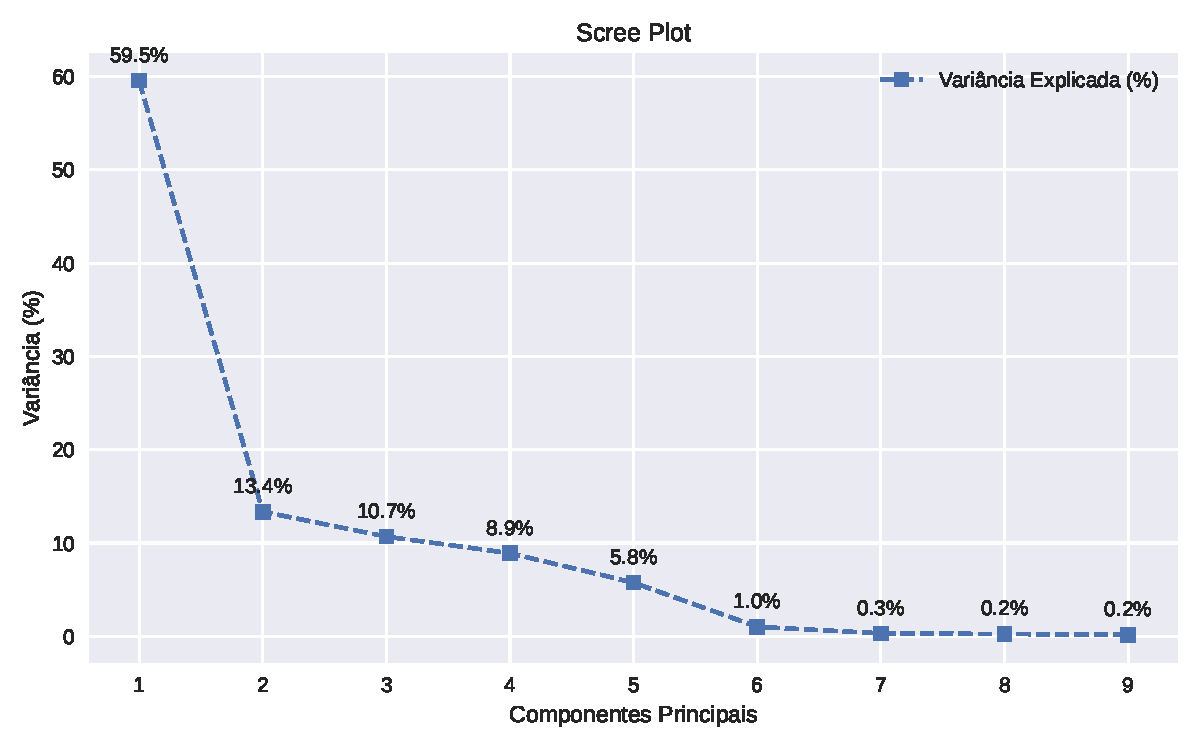
\includegraphics[width=1\linewidth]{images/PCA-screeplot.pdf}
    \caption{Scree Plot mostrando a variância explicada por cada componente principal (PCA). Cada ponto representa a porcentagem da variância total capturada pela respectiva componente, permitindo identificar quantos PCs são suficientes para representar a maior parte da informação dos dados.}
    \label{fig:screeplot}
\end{figure}

\begin{figure}[H]
    \centering
    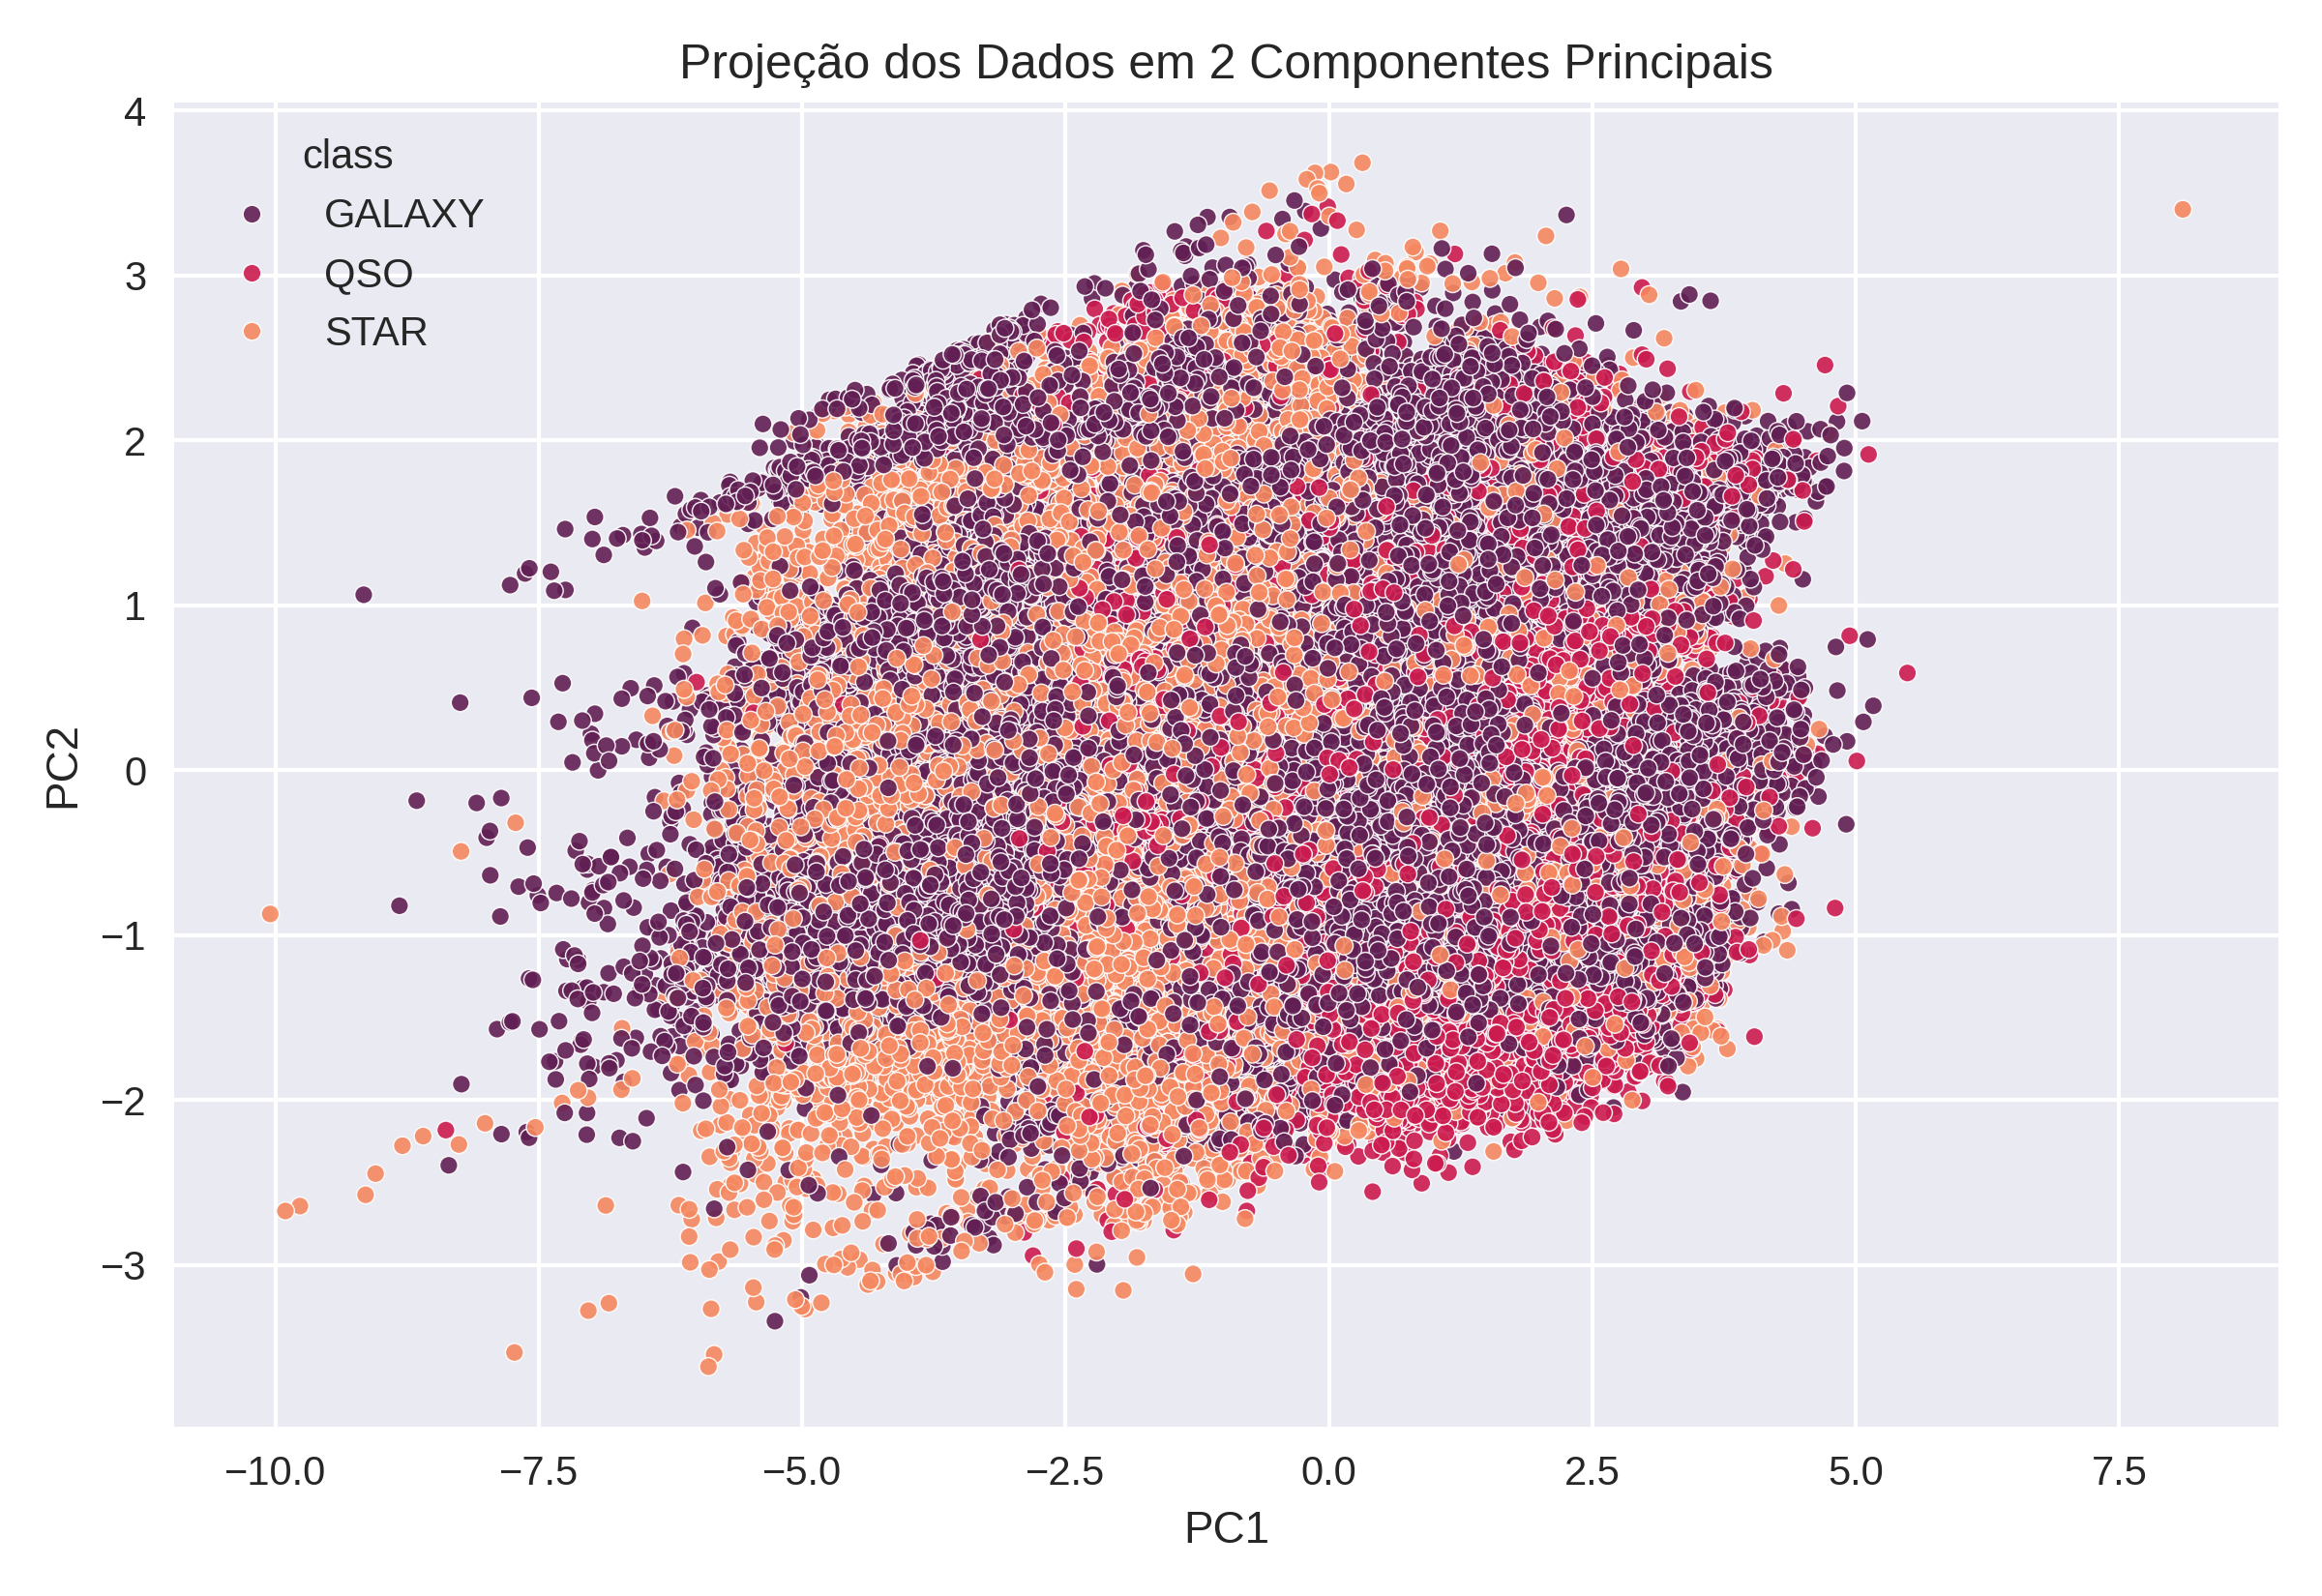
\includegraphics[width=1\linewidth]{images/2PC-projection-scatterplot.png}
    \caption{Projeção dos dados nas duas primeiras componentes principais (PC1 e PC2). Cada ponto representa uma amostra no espaço reduzido pelo PCA, permitindo a visualização de dispersão. Visualiza-se sobreposição de agrupamentos.}
    \label{fig:scatter_pca}
\end{figure}


\begin{thebibliography}{00}

\bibitem{b1} G. Kauffmann and M. Haehnelt, “A unified model for the evolution of galaxies and quasars" Mon. Not. R. Astron. Soc., vol. 311, pp. 576–588, 2000.

\bibitem{b2} E. M. Burbidge, G. R. Burbidge, W. A. Fowler, and F. Hoyle, “Synthesis of the elements in stars,” Rev. Mod. Phys., vol. 29, no. 4, pp. 547–650, Oct. 1957.

\bibitem{b3} Sloan Digital Sky Survey, “Instruments," SDSS, 2025. [Online]. Available: https://www.sdss.org/instruments/.

\bibitem{b4} Abdurro’uf, N., K. Accetta, C. Aerts, et al. 2022. “The Seventeenth Data Release of the Sloan Digital Sky Surveys: Complete Release of MaNGA, MaStar, and APOGEE-2 Data.” Astrophysical Journal. Supplement Series 259, no. 2: 1–39.

\bibitem{b5} E. Veloso, G. Júnior e R. Rego, “Modelo Perceptron Multicamadas para Classificação de Estrelas, Quasares e Galáxias,” Universidade Federal Rural do Semi-Árido, Pau dos Ferros, RN, Brasil, 2023.

\bibitem{b6} D. Chatterjee and P. Ghosh, “Redshift-Agnostic Machine Learning Classification: Unveiling Peak Performance in Galaxy, Star, and Quasar Classification (Using SDSS DR17),” Astronomische Nachrichten, 2025.

\bibitem{b7} D. Omat, O. Otey, and A. Al-Mousa, “Stellar Objects Classification Using Supervised Machine Learning Techniques,” in Proc. 2022 Int. Arab Conf. on Information Technology (ACIT), Amman, Jordan, 2022.

\bibitem{b8} F. R. Llorella and J. A. Cebrián, “Exploring Symbolic Regression and Genetic Algorithms for Astronomical Object Classification,” arXiv preprint arXiv:2503.09220 [astro-ph.GA], Mar. 2025.


% PCA ------------------------------
\bibitem{pca} H. Abdi and L. J. Williams, “Principal component analysis,” Wiley Interdisciplinary Reviews: Computational Statistics, vol. 2, no. 4, pp. 433–459, 2010.



\end{thebibliography}



\end{document}
